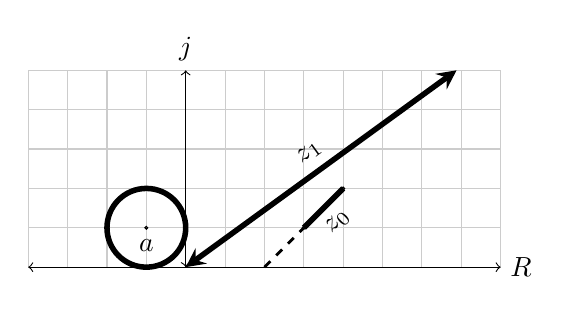
\begin{tikzpicture}[scale=0.5]
    \draw [thin,gray!40] (-4,0) grid (8,5);
    \draw[<->] (-4,0)--(8,0) node[right] {$R$};
    \draw[<->] (0,0)--(0,5) node[above]{$j$};
    \coordinate (a) at (-1,1);
    \coordinate (b) at (3,1);
    \coordinate (c) at (4,2);
    \coordinate (d) at (-5,-3.634);
    \coordinate (e) at (6.88,5);
    \coordinate (f) at (2,0);
    
    \draw[line width=2pt,black] (a) circle(1) node[anchor=north]{$\Vec{a}$};
    \draw[black] (a) circle(1pt) node[anchor=south]{};
    \draw[black] (b) circle(1pt) node[anchor=south]{};
    \draw[black] (c) circle(1pt) node[anchor=south]{};
    \draw[line width=2pt,black,-] (b)--(c) node[midway, below, sloped]{$z_0$};
    \draw[line width=2pt,black,stealth-stealth] (0,0)--(e) node[midway,above,sloped]{$z_1$};
    \draw[line width=1pt,black,dashed] (f)--(b) node[midway, above, sloped]{};
\end{tikzpicture}
\caption*{Figuras sin escalar}